q
\chapter{Experiment Result and Discussion}

This chapter provides the result and the analysis of the experiment. three hypothesis are analyzed;
\begin{itemize}
  \item{Do participant experience the failure of prospective memory while using the smartphone?}
  \item{Is failure of prospective memory is more likely to happen with two intentions rather than one; intentional load matters}
  \item{What is the effect of notification to prospective memory error}
  \item{Does mentaly moving through event boundary increase the likeliness to experience failure of prospective memory?}
\end{itemize}

\section{Prospective memory error on smartphone}

\subsection{Experiment result}
In these expriment the data from the participants from the three studies is combined.
Table \ref{fig:affirmationTable} shows who many participants believe that they have experienced prospective memory error,
and how many participant actually experience the prospective memory error during the experiment.
The participant were asked if they believe that they had experince prospective memory error using the first question on the Table \ref{tab:demographicQuestion}.
Actual experience of memory error was calculated by looking if the people forget the questions during the experiment.

%The prospective memory error on the experiment is presented by the lost of intention during the study.
% The first column shows the affirmation on the prospective memory. the number is obtained by asking the participants \textit{"Often people go into a room to do something.  Though they know they intended to do something, they lose track of what they wanted to do.
% This same sort of thing can happen when using a smart phone, as well.  During the study,
% you may have clicked on a link, gone to the website, and then forgot what you intended to look up.  Did that happen to you at all during this study?"} on the post question phase during the experiment.
% While the second column is obtained by counting how many participant forget the question and chosed to look at the question again (lookback) during an experiment.
% The last column shows the total number of the participant participated on each study.
 %or forget the question during the experiment.

\subsection{Discussion}
% As seen in figure \ref{fig:demo1Study1}, \ref{fig:realdemo1Study1}, \ref{fig:demo1Study2}, \ref{fig:realdemo1Study2}, \ref{fig:demo1Study3}, \ref{fig:realdemo1Study3}, the left
% pie chart shows percentage of participant who think they are experiencing prospective memory error, and on the right side shows the percentage of participant who experience
% the prospective memory failure during the experiment.

Most of the participant did not believe that they have experienced the prospective memory error
. In contrast, the output shows that  almost 70\% of the participant actually experienced the prospective memory error.
We can agrue that the participant made an intention for looking the answer before clicking the answer link, but after reading the answer page
they lost their original intention.
As a result they forget the content of the question, and they experience prospective memory error.
This shows that while using a smartphone a person has a high probability of experiencing prospective memory error.
This experiment support the result of Prof. Richard alan Carlson's experiment.

% \begin{table}[]
% \centering
% \label{my-label}
% \begin{tabu}{|X[3,c]|X[3,c]|X[3,c]|}
% \hline
% \multicolumn{3}{|c|}{Study 1}                                                                             \\ \hline
% Affirmation of prospective memory error & \begin{tabular}[c]{@{}l@{}}Forget the questions \end{tabular} & Total Person \\ \hline
% 0                      & 3                                                                 & 4            \\ \hline
% \multicolumn{3}{|c|}{Study 2}                                                                             \\ \hline
% Affirmation of prospective memory error & Forget the questions  & Total Person \\ \hline
% 5                      & 8                                                                 & 11           \\ \hline
% \multicolumn{3}{|c|}{Study 3}                                                                             \\ \hline
% Affirmation of prospective memory error & Forget the questions                                            & Total Person \\ \hline
% 2                      & 2                                                                 & 3            \\ \hline
% \end{tabu}
% \caption{Participant affirmation and their experiment result on prospective memory error on smartphone}
% \label{fig:affirmationTable}
% \end{table}


\begin{table}[]
\centering
\small
\footnotesize
\begin{tabu}{|X[6,l]|X[2,c]|X[2,c]|X[2,c]|}
\hline
                                                                           & Experiment 1 (n=4) & Experiment 2 (n=11) & Experiment 3 (n=3) \\ \hline
How many participant believe they have experience prospective memory error & 0                  & 5                   & 2                  \\ \hline
How many participant actually experienced prospective memory error          & 3                  & 8                   & 2                  \\ \hline
\end{tabu}
\caption{Number of participant from all the studies who believe they have experince prospective memory error and the actual result of the experiment}
\label{fig:affirmationTable}
\end{table}



\section{The effect of multiple intention}

\subsection{Experiment result}
This section shows the result from the second study. On the second study, one or two question are presented to the participant randomly.
A participant intention is to find for the answer. Thus the number of question presented is the number of intention need to be retained by the participant.
Using the result we are trying to see  if an increasing the number of intention will make people more likely to experience failure of prospective memory (is the intentional loads matter ?).
Table \ref{fig:oneTwoQuestionForget} shows the total number of times the participant forget the question on the experiment.
It shows that when the participant presented with two question they are 75\% more probably to forget the
question rather than presented by one question.

Figure \ref{fig:TTFA_oneTwoQues} shows how long in millisecond each participants need to write the answer (TTLFA).
The horizontal axis is the 11 participants and the vertical axis shows the duration of writing.
 It shows that 63\% (7 out of 11) have longer time writing the answer if two questions are presented each time.

All the participants data are combined and group between one or two question. Figure \ref{fig:TTLFA_oneTwoQuesGeneral} shows the mean of the writing time between both group.
It shows that if two questions are presented then it will take longer time for the people to recall content of the answer thus make the writing time longer.

Figure \ref{fig:lookingAnswer_oneOrTwo} shows the average time each participant spent on finding the answer in the answer page.
 The top plot was calculated on the first time they see the answer page.
 While the lower plot was calculated the second time they see the answer page, after they decide to see the question again (loopback).
Surprisingly the top plot shows that almost half of the particpants (4 out of 11) spent significantly longer time for one questions.
However. the lower plot shows that most of the participant spent longer time if two question are presented .

\subsection{Discussion}

The result of this study shows that the amount of intentional loads are important component on prospective memory. Based on the table \ref{fig:oneTwoQuestionForget}, a person is more probable to experience
prospective memory error if the amount of the intention is higher.

Furthermore, the result on figure \ref{fig:TTFA_oneTwoQues} and figure \ref{fig:TTLFA_oneTwoQuesGeneral} shows that the increasing amount intentional loads also make the person harder to recall the content of the intention.
 % On this analysis, this intention is different with the first intention which looking for the answer,
On this analysis the intention is to answer the question and it's formed after the participant found the answer on the answer page.
The recall time is presented as the time participant write the answer.

\todo[inline]{FUCK THIS SHIT}
Based on figure \ref{fig:lookingAnswer_oneOrTwo}, the increasing amount of intention also increase the time
the participant spent on looking for the answer.


These result shows that the number of intention decrease their cognitive performance which result on the likeliness of experiencing the failure of prospective memory.
This probably because the increase of intentions will reduce the level of attention given on the task, and make
the participant take a longer time to find the answer.


% Please add the following required packages to your document preamble:
% \usepackage{multirow}
\begin{table}[!h]
\centering
\begin{tabular}{|l|l|l|}
\hline
\multirow{2}{*}{Participant} & \multicolumn{2}{l|}{How many times the participant forget the question} \\ \cline{2-3}
                             & One question                  & Two question                 \\ \hline
1                            & 0                             & 1                            \\ \hline
2                            & 1                             & 2                            \\ \hline
3                            & 0                             & 2                            \\ \hline
4                            & 1                             & 0                            \\ \hline
5                            & 0                             & 0                            \\ \hline
6                            & 0                             & 0                            \\ \hline
7                            & 1                             & 0                            \\ \hline
8                            & 0                             & 1                            \\ \hline
9                            & 0                             & 0                            \\ \hline
10                           & 0                             & 2                            \\ \hline
11                           & 1                             & 2                            \\ \hline
Sum                          & 4                             & 10                           \\ \hline
\end{tabular}
\caption{The number of question the participants forget}
\label{fig:oneTwoQuestionForget}
\end{table}

% Hampir 75\% dari kelupaan adalah two questions.
%
% then show that TTLFA time they write the answer also longer
% then show that using two question make people look at the answer longer time,
% turns out not. but most of the time participant look again the answer for two question

\begin{figure}[!h]
\centering
\begin{minipage}{.5\textwidth}
  \centering
  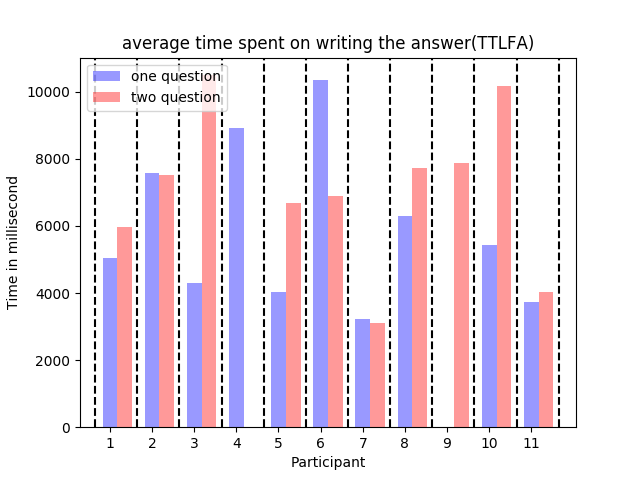
\includegraphics[scale=0.5]{TTFLA_each_participant}
  \captionsetup{justification=centering}
  \captionof{figure}{Average time each participant filling the answer}
  \label{fig:TTFA_oneTwoQues}
\end{minipage}%
\begin{minipage}{.5\textwidth}
  \centering
  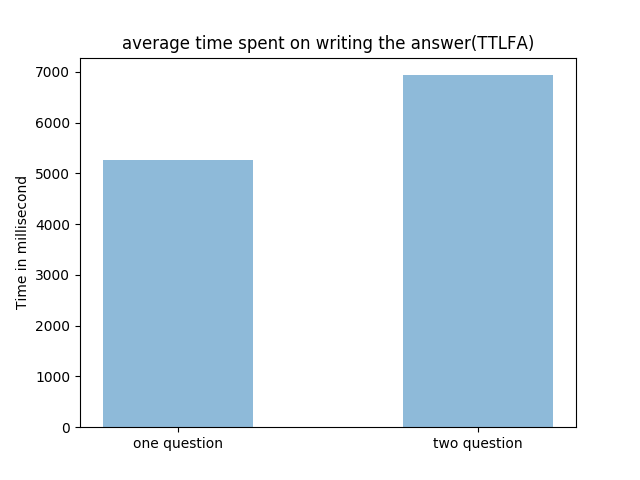
\includegraphics[scale=0.5]{TTLFA_general}
  \captionsetup{justification=centering}
  \captionof{figure}{Average time of all the participants filling the answer}
  \label{fig:TTLFA_oneTwoQuesGeneral}
\end{minipage}
\end{figure}


\begin{figure}[!h]
\begin{center}
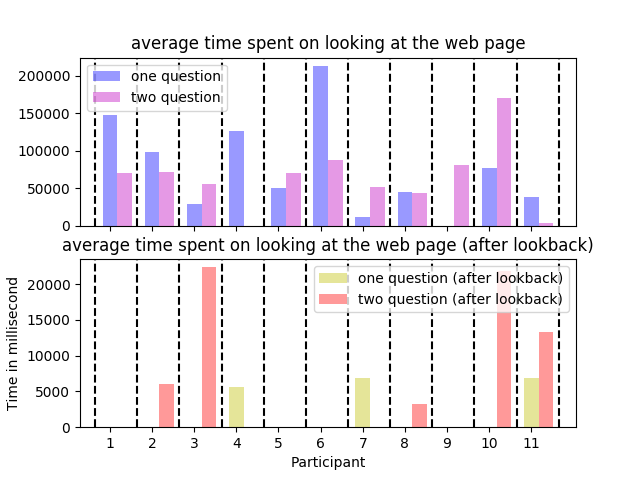
\includegraphics[scale=0.86]{visitedLink_each_participant}
\end{center}
\captionsetup{justification=centering}
\caption{Average time in spent finding for an answer between one or two questions}
\label{fig:lookingAnswer_oneOrTwo}
\end{figure}


% \begin{table}[]
% \centering
% \caption{My caption}
% \label{my-label}
% \begin{tabular}{|l|l|l|l|l|l|l|l}
% \cline{1-7}
% \multirow{2}{*}{Question}           & \multicolumn{2}{l|}{Study 1} & \multicolumn{2}{l|}{Study 2} & \multicolumn{2}{l|}{Study 3} &  \\ \cline{2-7}
%                                     & Yes           & No           & Yes           & No           & Yes           & No           &  \\ \cline{1-7}
% Experience prospective memory error & 0             & 4            & 5             & 6            & 2             & 1            &  \\ \cline{1-7}
% Forget about the answer             & 2             & 2            & 4             & 7            & 0             & 3            &  \\ \cline{1-7}
% \end{tabular}
% \end{table}

% Please add the following required packages to your document preamble:
% \usepackage{multirow}


\subsection{The effect of notifiaction on the intention}
\subsection{Experiment Result}
Table \ref{tab:notifiactionNumber} shows the time participant spent on writing the answer (TTLFA), average time finding for the answer
and the percentage of lookback on each number of notification shown up.
It show that by increasing the number of notification make people spent more time writing the answer and finding for the answer.

\begin{table}[]
\centering
\begin{tabular}{|l|l|l|}
\hline
\multicolumn{3}{|c|}{No Notification}                      \\ \hline
TTFA    & Average time looking  at answer page & Lookback percentage \\ \hline
6267.68 & 59875.22 millisecond                   & 17\%                   \\ \hline
\multicolumn{3}{|c|}{One Notifications}                     \\ \hline
TTLFA   & Average time looking at answer page  & Lookback frequency \\ \hline
7292.87 & 69517.0 millisecond                    & 11\%                 \\ \hline
\multicolumn{3}{|c|}{Two Notifications}                      \\ \hline
TTLFA   & Average time looking at answer page  & Lookback frequency \\ \hline
7304.87 & 76699.16  millisecond                   & 21\%                 \\ \hline
\end{tabular}
\caption{The experiment result on each notification number}
\label{tab:notifiactionNumber}
\end{table}

\subsection{Disscussion}
These result shows that the notification influence the intention, but it doesn't increase the probability of prospective memory error.
Table \ref{tab:notifiactionNumber} shows that the increasing number of notification make people harder to recall the content of the memory.
If the notification popped up when the participant presented with the question. The notification probably lower the level of attention thus make
the intention is not framed perfectly. But if the notification popped up when the participant find the answer, this can mean that the notification attenuate the intention,
even though it's correctly framed before. As a result the participant can experience the detached intention \citep{Reason1984}.

In addition, if we consider the notification as an event boundary. However, Table \ref{tab:notifiactionNumber} shows
that the notification quantity is not linear with the percentage of forgetting the question.
So it shows that mentaly moving through event boundary will have no effect on the prospective memory error.

\subsection{Event boundary on prospective memory}
\subsection{Experiment Result}
The bar chart \ref{fig:lookingAnswer_lookback} shows the average time (in millisecond) the participants spent finding for the answer on the answer page.
The chart shows that if the participant forget the question and decide to see it again (lookback), they spent longer time finding the answer compare to if they don't forget the question(non-lookback).
The bar chart \ref{fig:freq_study1} and \ref{fig:freq_study3} shows the frequency of looking the question again (lookback) for all questions  between first and the third study.
It shows that the peole more frequently do a lookback on third study rathern than on study one.
The bar chart \ref{fig:aveTime_study1} and \ref{fig:aveTime_study3} shows the time spent looking for the answer for all the questions between first and the third study.
It shows that the participant spent longer time to look at the answer and they spent longer time to look at the answer again after the do lookback.
\begin{figure}[!h]
\begin{center}
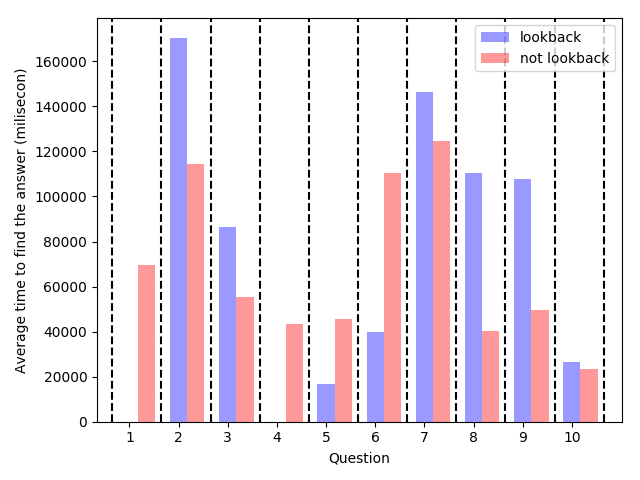
\includegraphics[scale=0.86]{lookback_and_reading_time_studyAll}
\end{center}
\captionsetup{justification=centering}
\caption{Average time in spent looking for an answer between lookback and non-lookback in all studies}
\label{fig:lookingAnswer_lookback}
\end{figure}

\begin{figure}[!h]
\centering
\begin{minipage}{.5\textwidth}
  \centering
  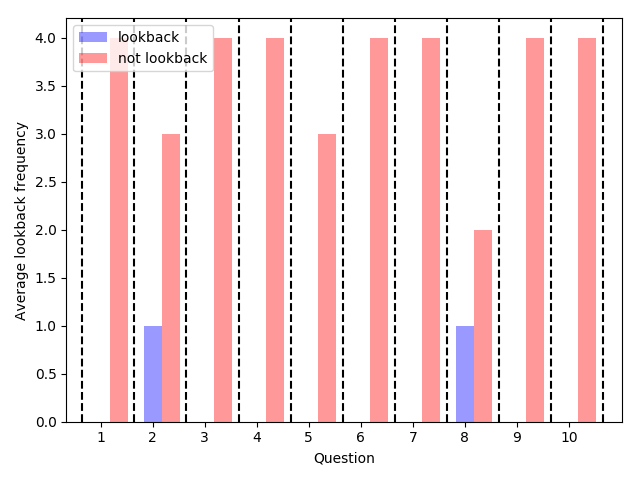
\includegraphics[width=\textwidth]{frequency_lookback_study1}
  \captionsetup{justification=centering}
  \captionof{figure}{Frequency of lookback of the participant on study 1}
  \label{fig:freq_study1}
\end{minipage}%
\begin{minipage}{.5\textwidth}
  \centering
  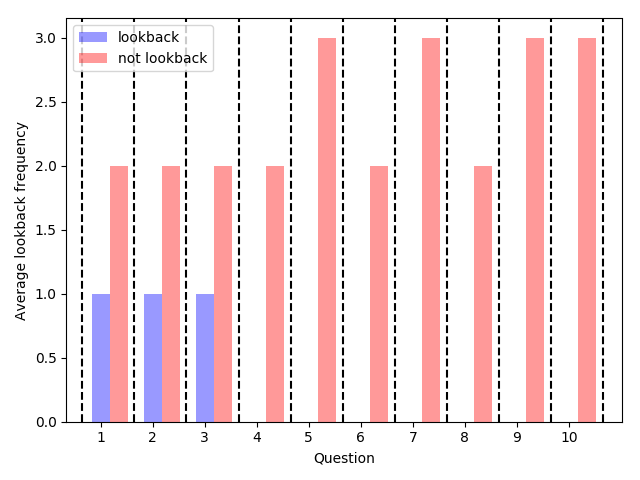
\includegraphics[width=\textwidth]{frequency_lookback_study3}
  \captionsetup{justification=centering}
  \captionof{figure}{Frequency of lookback of the participant on study 3}
  \label{fig:freq_study3}
\end{minipage}
\end{figure}

\begin{figure}[!h]
\centering
\begin{minipage}{.5\textwidth}
  \centering
  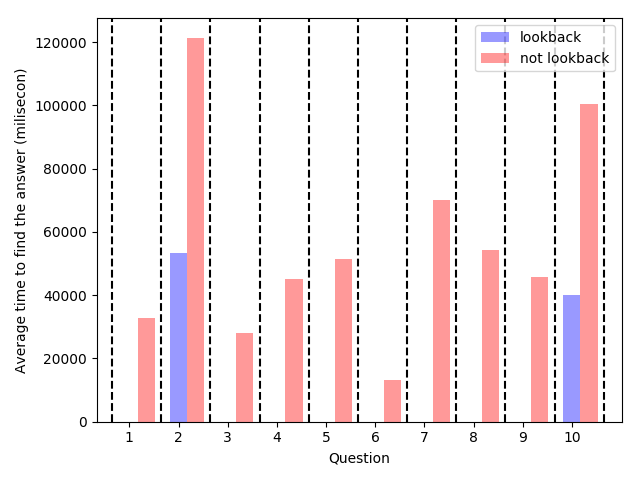
\includegraphics[width=\textwidth]{lookback_and_reading_time_study1}
  \captionsetup{justification=centering}
  \captionof{figure}{Average time each participant looking for the answer in study 1}
  \label{fig:aveTime_study1}
\end{minipage}%
\begin{minipage}{.5\textwidth}
  \centering
  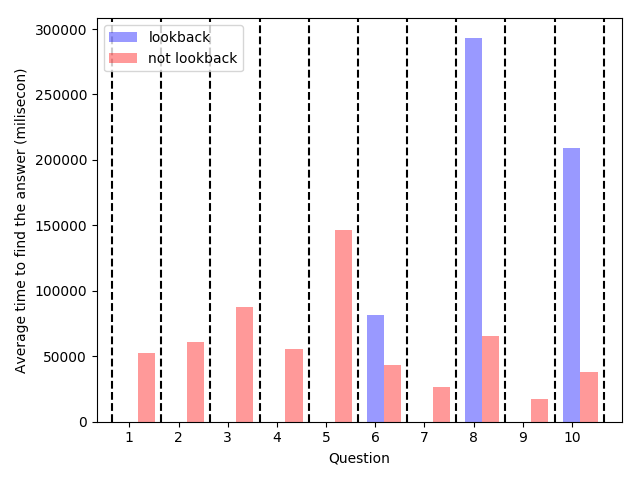
\includegraphics[width=\textwidth]{lookback_and_reading_time_study3}
  \captionsetup{justification=centering}
  \captionof{figure}{Average time of all the participants looking for the answer in study 3}
  \label{fig:aveTime_study3}
\end{minipage}
\end{figure}

\subsection{Discussion}
The result of the bar chart \ref{fig:lookingAnswer_lookback}  shows that the paricipant will more likely to experience prospective memory error if they read longer than the average time
of the participant who do not experience memory error. The participant probably miss the answer or read some interesting information which
make them read longer, then they experience lost intention \cite{Reason1984} as a result they experience  prospective memory error.
We can argue that the participant experience the event boundary which is moving from the android application to the answer page for looking to the answer.
The time spent on reading represent the level of immersion people have on after the event boundary. So the type and the level of immersion of the task after the event
boundary hold a signifact factor on deciding if the person willl experience failure of prospective memory or not.

To understand the effect of physical transition through event boundary we try to investigate the frequency of prospective memory error between first on the third study.
Bar chart \ref{fig:freq_study1} and \ref{fig:freq_study3} shows that the participant on the third study forget the question more frequently than the first study. However,
it cannot show strong correlation between physically moving through another room with prospective memory failure phenomena.
Because the sample is very small so we cannot make any solid conclusions on whether the physical transtition of the event boundary will increase the probability of a person to experience
prospective memory error. However, by looking at bar charts \ref{fig:aveTime_study1} and \ref{fig:aveTime_study3} we can see that the physical transtition result on the longer time for people to read and find the answer.
This shows that the physical transition decrease the capability of cognitive ability while doing this experiment.
